% Chapter Template

\chapter{Data gathering and processing}
\label{Chapter2}
Data were sourced from several streams. The Icelandic Meteorological Office (IMO) provided measurements from weather stations across Iceland, NWP data were downloaded from the Copernicus Arctic Regional Reanalysis dataset (CARRA), and finally a land-elevation model was also provided by the IMO.

\section{Automatic Weather Station Data}

IMO provided measurements from \nStationsMin weather stations across Iceland. The measurements that met the filtering criteria began in \startDateVedur and ended in 2023. Of these \nStationsMin stations, \nVedurMin were from the IMO, with the anemometer at 10~m above ground, while the remaining \nVGMin stations were from \href{https://www.vegagerdin.is/}{the Icelandic Road and Coastal Administration (IRCA)}, with the anemometer at 6–7~m above ground \cite{vegagerdin_postur}. The locations of these weather stations are shown in Figure \ref{fig:aws_map}.

Data from these automatic weather stations (AWS) are stored in hourly files, which aggregate the original 10-minute files; measurement errors—unrealistic spikes known as “nails”—have been removed in most cases. Each record contains the following information: date and time; station number (convertible to coordinates using another dataset of Icelandic meteorological stations); average wind speed (\(f\)); wind gust (\(f_g\)); standard deviation of the wind gust; wind direction (\(d\)); and standard deviation of the wind direction.

These measurements began at the end of the 20th century with the installation of the first AWSs, and more stations have been added in subsequent decades.

\begin{figure}
    \centering
    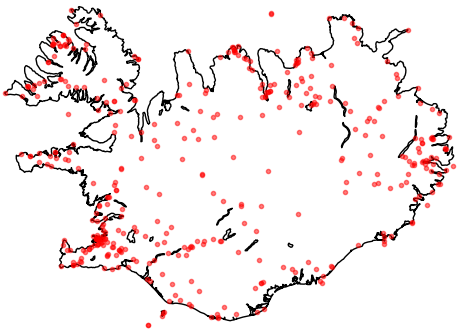
\includegraphics[scale = 1]{Figures/stationsOverIceland_2024-05-16_stripped_to_frame.png}
    \caption[Locations of automatic weather stations in Iceland]{Locations of all 412 stations that were looked at in this study. Most of these were from IMO but over a hundred were from IRCA. IMO anemometers are placed at 10 meters above ground, while IRCA ones are placed at 6--7 meters above ground.}
    \label{fig:aws_map}
\end{figure}

\section{CARRA Data}
CARRA is a high-resolution atmospheric reanalysis produced by the Copernicus Climate Change Service and run by ECMWF. It covers two regions, a west region covering Greenland and Iceland and an east region covering the European Arctic. It has a 2.5 km horizontal resolution and dates from 1991 to the present, with monthly updates. CARRA provides three-hourly analysis fields and short-term forecasts (hourly for lead times under 6 h and three-hourly beyond) of surface and near-surface variables—wind, temperature, pressure, precipitation, etc. It is based on the HARMONIE-AROME limited-area NWP model, forced at its boundaries by ERA5 (ECMWF Re-Analysis v. 5) and enhanced by local observations to better represent complex terrain, land–sea contrasts, and sea-ice processes. It is updated monthly, with a latency of 2-3 months\cite{carra_information}.

The CARRA dataset covers all the IMO observations that fulfill criteria of consistent availability – the oldest observation is from \startDateVedur. The CARRA-West region covers a vastly larger area than the area of interest. This leads to having to store a large amount of data. To download CARRA data one has two options, a web interface or using an API client provided by CARRA. Using the API client is the only realistic option here, as there are thousands of requests made for different times. If using the API, it is possible to query a smaller area (such as a rectangular area around Iceland) given a set of coordinates, but this is not possible with the web interface.

The requests to the API were made at each available CARRA hour ([00, 03, 06, 09, 12, 15, 18, 21]) on a grid covering Iceland, for each available observation time. The downloaded data were interpolated to get values at the weather stations. CARRA contains several types of layers: single levels, model levels, height levels, and pressure levels. The data for this thesis was downloaded from height levels. They were requested at heights of 15, 250 and 500 meters above ground. For each point 4 parameters were requested, wind speed, wind direction, pressure, and temperature.

\section{Elevation data}
A GeoTIFF file containing Iceland’s elevation on a 20~m by 20~m grid was provided by the Icelandic Meteorological Office (IMO). The entire country is covered by this file, and its size is approximately 685\,MB.

The Python package \texttt{rasterio} is used, enabling rapid elevation lookup via its spatial indexing and affine‐transform capabilities. Elevation at specified geographic coordinates can be retrieved directly, and grid indices may be used for efficient access. Elevation for any exact location can be interpolated by fetching neighboring grid points.

\section{Combining data sources}

Three main data sources were used, each requiring querying, filtering, and merging to prepare the combined dataset. When handling hundreds of thousands of rows, code efficiency is essential: row-by-row iteration can increase execution time dramatically compared to vectorized operations.

The sources were provided in different formats: IMO measurement data in text files, elevation data in GeoTIFF, and CARRA reanalysis data in GRIB. To train the models, these datasets were combined into a single file using the IMO measurements as a reference. CARRA data are supplied on a rectangular grid with approximately 2.5~km spacing, while IMO observations are tied to specific station locations. Elevation data are on a 20~m by 20~m grid covering Iceland. Linear interpolation was applied to merge the sources.

\begin{figure}[h]
  \centering
  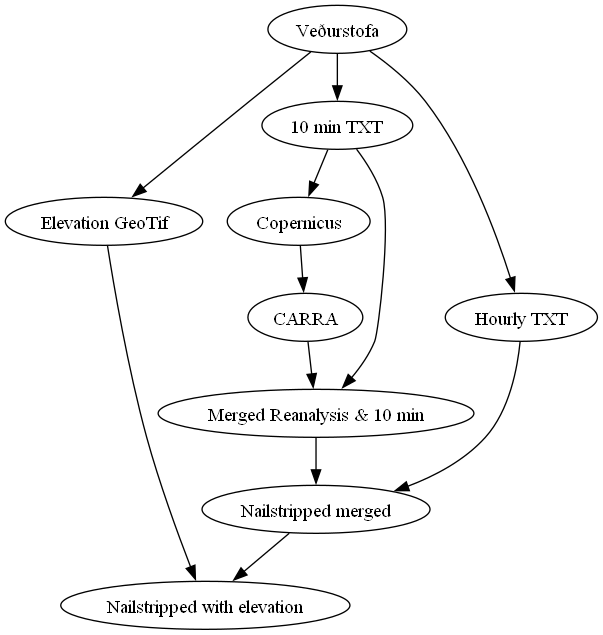
\includegraphics[scale=0.5]{Figures/data-preprocessing-flow-chart.png}
  \caption{Flow chart illustrating the data-combination workflow}
  \label{fig:data_preprocessing_flow_chart}
\end{figure}

The merging procedure, shown in Figure \ref{fig:data_preprocessing_flow_chart}, was as follows: for each AWS observation, a query was constructed for the CARRA API by specifying year, month, day, hour, and spatial extent. Because the API returns all specified days when queried by hour, and all specified months when queried by day, monthly queries were issued for only the required days, retrieving all eight three-hourly time points (00, 03, 06, 09, 12, 15, 18, and 21~UTC). After downloading the requested variables at the desired pressure levels, point values were interpolated and appended to a pandas dataframe. The monthly GRIB files were then discarded before proceeding to the next month. This strategy reduced storage needs from several terabytes to under one gigabyte.

Elevation values from the GeoTIFF were interpolated in the same manner: the four surrounding grid points were used in a linear interpolation to estimate the elevation at each station location. These interpolated values were included in the dataframe, since topography influences both average wind speed and gustiness \cite{GNP_vidtal}.

\section{Comparison of observed and reanalysis wind speed}

The error in reanalysis wind speed and measured wind speed can be significant. The absolute error increases as the measured wind speed increases, while the percentage wind speed decreases. A grouping of these errors by wind speed can be seen in Table \ref{table:measuredVSReanalysis_wind_speed}


\begin{table}[h]
    \caption[Comparison of measured and reanalysis wind speed]{Comparison of measured and reanalysis wind speed using mean absolute error (MAE) and mean absolute percentage error (MAPE). Note that for the computation of MAPE for ranges that otherwise include 0, 0 values have been excluded so as to prevent division by zero and exploding values. The comparisons are done using measured wind speed (at 10 meters above ground for IMO and 6-7 meters above ground for IRCA) and reanalysis wind speed at 15 meters above ground.}
    \label{table:measuredVSReanalysis_wind_speed}
    \centering
    \begin{tabular}{ccc}%c}
        \toprule
        f & n & MAE \\%& MAPE \\
        \midrule
        $[0;5[$ & 6.2e6 & 2.1 \\%& 1.6\\
        $[5;10[$ & 4.2e6 & 2.2 \\%& 0.3\\
        $[10;15[$ & 1.5e6 & 2.5 \\%& 0.2\\
        $[15;20[$ & 3.9e5 & 3.0 \\%& 0.2\\
        $[20;25[$ & 8.4e4 & 4.0 \\%& 0.2\\
        $[25;\infty[$ & 2.0e4 & 6.6 \\%& 0.2\\
        $[0;\infty[$ & 1.2e7 & 2.2 \\%& 1.0\\
        \bottomrule
    \end{tabular}
\end{table}

Another thing to look at is the distribution of error by station, both in terms of their coordinates and number of measurements. Looking at Figure \ref{fig:station_mae_distribution}, this distribution can be seen.

\begin{figure}
    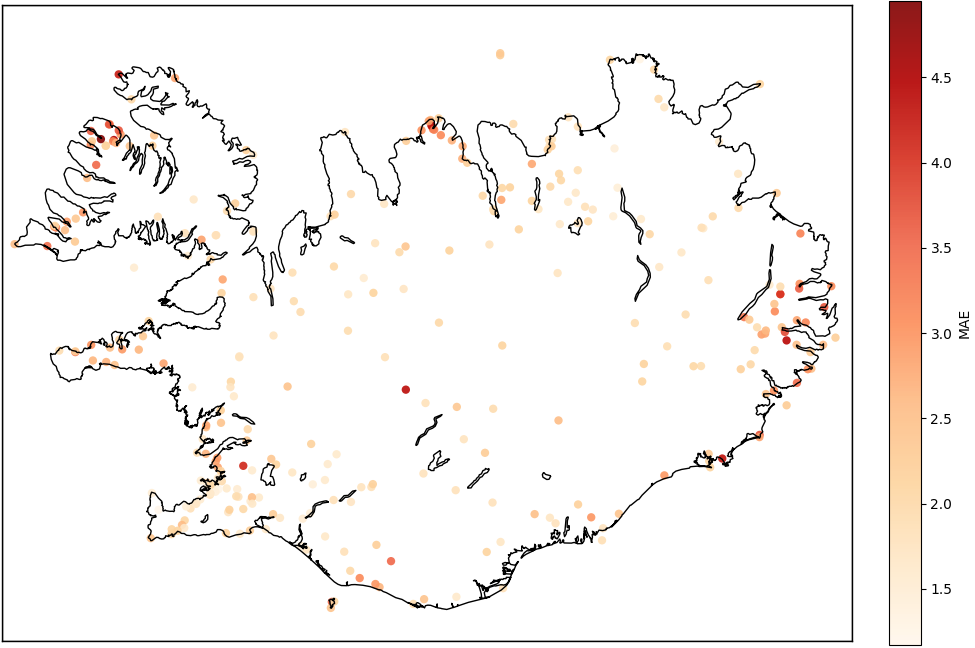
\includegraphics[scale=0.6]{Figures/MAEoverIceland.png}
    \caption[Distribution of mean absolute errors by station]{The distribution of mean absolute errors by station. Using mean absolute error instead of mean absolute percentage error allows for all points to be used. Mean absolute percentage error can only be used if 0 values are ignored.}
    \label{fig:station_mae_distribution}
\end{figure}

Table \ref{table:station_mae_distribution} shows the 5 best and worst stations in terms of MAE.

\begin{table}[h]
    \caption[Mean absolute difference of measured wind speed and reanalysis wind speed at select stations]{Mean absolute error for reanalysis wind speed as compared to measured wind speed, for the five stations with the highest difference and the five stations with the lowest difference.}
    \label{table:station_mae_distribution}
    \resizebox{\textwidth}{!}{
    \centering
    \begin{tabular}{cccc}
        \toprule
        Station & Number of measurements & MAE & Location \\
        \midrule
        1470 & 6.8e3 & 1.17 & Reykjavík Háahlíð \\
        1350 & 5.2e4 & 1.18 & Keflavíkurflugvöllur \\
        1482 & 1.4e4 & 1.23 & Reykjavík Víðidalur \\
        4921 & 1.3e4 & 1.29 & Rif á Melrakkasléttu \\
        1477 & 5.6e4 & 1.29 & Reykjavíkurflugvöllur\\ \hdashline[0.5pt/1pt]
        35553 & 4.0e3 & 4.30 & Almannaskarð - göng\\
        6745 & 1.5e4 & 4.36 & Kerlingarfjöll - Ásgarðsfjall\\
        35978 & 7.9e3 & 4.40 & Fáskrúðsfjarðargöng suður\\
        2640 & 1.6e3 & 4.51 & Seljalandsdalur\\
        32635 & 3.2e4 & 4.95 & Botn í Súgandafirði\\
        \bottomrule
    \end{tabular}
    }
\end{table}

\section{Data Structure}

Once data has been retrieved for all three sources and processed, including interpolating values, it needs to be made ready to use by the model, for both training, validation and test. The starting point is a dataframe that contains measured information from AWS. This includes the average wind, the wind gust, wind direction along with the station number and coordinates. When selecting the CARRA data certain height levels are chosen. These present as separate lines in the CARRA dataframe. Information for one observation is represented in as many lines as height levels requested in the reanalysis data. These rows need to be combined on the position (the weather station). When this is done it is possible to combine the AWS IMO data and CARRA reanalysis data on the location and time columns. The last data source is the elevation. A circle sector upwind is looked at. In any case the points, that represent these sections, were selected as shown in Code Listing \ref{code:sectorElevation}. A range of angles are defined based on the wind direction $d$ at some distance from the given point. This means that the resultant points (equal in number to the length of angleRange by k) from arcs at several distances from the given weather station.

\begin{lstlisting}[style = Python, caption = {Sector elevation points generated}, label = code:sectorElevation]
angles = [(angle + (90 - d)) * pi/180 for angle in angleRange]
length_rng = [(exp(i * log(n + 1)/ k) - 1) * 1000 
                for i in range(1, k + 1)]
points = np.array([[(X + l * cos(angle), Y + l * sin(angle))
                    for angle in angles] for l in length_rng])   
\end{lstlisting}

The result is a dataframe that has measured data from AWS, which gives us our target, reanalysis data from CARRA, which gives us weather variables to train on, and finally elevation points in the landscape to include in our training data. An example of what the data looks like can be seen in Table \ref{table:trainDataExample}.

\begin{table}[h]
    \caption[An example of data structure used to train model]{An example of data structure used to train model. Data points include the derived variables Richardson number ($Ri$) and Brunt-Väisäla frequency ($N$) (defined below), the elevation of the station, direction of wind and relative direction of the wind (twd, that is the direction of the wind relative to center of Iceland), along with some combination of wind speed, pressure and temperature at the different height levels. Finally there are the elevation points around a given station, where the elevation is relative to the station.}
    \label{table:trainDataExample}
    \resizebox{\textwidth}{!}{
    \centering
    \begin{tabular}{cccccccccc}
        \toprule
        Ri & $N^2$ & station elevation & twd & $ws_{15}$ & $wd_{15}$ & $t_{15}$ & $p_{15}$ & $elevation_0$ & \dots\\
        \midrule 
        -1.18e+00 &  2.67e+04 & 100 & 1.5 & 10 & 5 & 0 & 100 & 2 & \dots\\
        \bottomrule
    \end{tabular}
    }
\end{table}

Looking at Table \ref{table:trainDataExample} note that the first two columns represent two variables that describe the stability of the air. These are the Richardson number ($Ri$)\cite{richardson_number_skybrary} and Brunt–Väisälä frequency ($N$)\cite{brunt_vaisala_freq_eumtrain}, and are calculated using Equations (\ref{eqn:Ri}) and (\ref{eqn:N})\cite{mean_gust_HA_HO}. These values are calculated using reanalysis data at two different height levels. Thus $Ri$ refers to the Richardson number calculated between height levels 15m and 500m. Exactly the same notation is used with the Brunt–Väisälä frequency, except the square is used.

\begin{equation}
    \label{eqn:Ri}
    Ri = \frac{g \cdot dT \cdot dz}{T_{\textrm ave} \cdot dU^2} \unit{[]}
\end{equation}

\begin{equation}
    \label{eqn:N}
    N = \sqrt{\frac{g \cdot dT }{T_{\textrm ave} \cdot dz}} \unit{[Hz]}
\end{equation}

Here, $g$ is the acceleration due to gravity, $dT$ is the temperature difference between the two height levels, $dz$ is the elevation difference, $T_{\textrm ave}$ is the average temperature (that is the average of the two temperatures in the height levels) and $dU$ is the wind speed difference between the two height levels. Both of these numbers provide some insight about the stability of the air. A lower value for the Richardson number indicates a higher turbulence. A typical range of values could be between 0.1 and 10, with values below 1 indicating significant turbulence\cite{richardson_number_skybrary}. When the square of the Brunt-Väisälä frequency is negative, then the air is unstable (an air parcel will move away from its original position)\cite{brunt_vaisala_freq_eumtrain}. These are derived factors from the reanalysis data and as such there shouldn't be a significant information gain using $Ri$ and $N$ as opposed to having the raw data. However, including these factors instead of every reanalysis variable requested might speed up training as well as making the model more easily explainable with the use of Shapley values or other tools for explainability. Using Shapley a feature importance value is attributed to a given feature by creating all possible permutations of any possible length (up to number of features) and seeing how the predictions are skewed when the given parameter is included or excluded. This needs to be done for all parameters. The time complexity of this is very high ($2^n$ coalitions)\cite{shapley_information}. Most implementations use some approximations, which still can take a considerable amount of time for models with a high parameter count and many examples. The Richardson number includes the difference in wind speeds in the denominator. In certain cases, where the difference in wind speed between two levels is very, can blow up to infinity. This can cause problems and distort the predicitons.

\section{Data distribution}

The CARRA data is reanalysis and as such might have a bias or some systemic distortion when compared to the measured data. The distribution of the observed and reanalysis wind speed can be seen in Figure \ref{fig:obs_carra_wind_speeds}. Looking at the figure, the reanalysis wind tends to be higher even though the distribution is similar. 

\begin{figure}[ht]
    \centering
    % First subfigure (top)
    \begin{subfigure}[b]{0.8\textwidth}
        \centering
        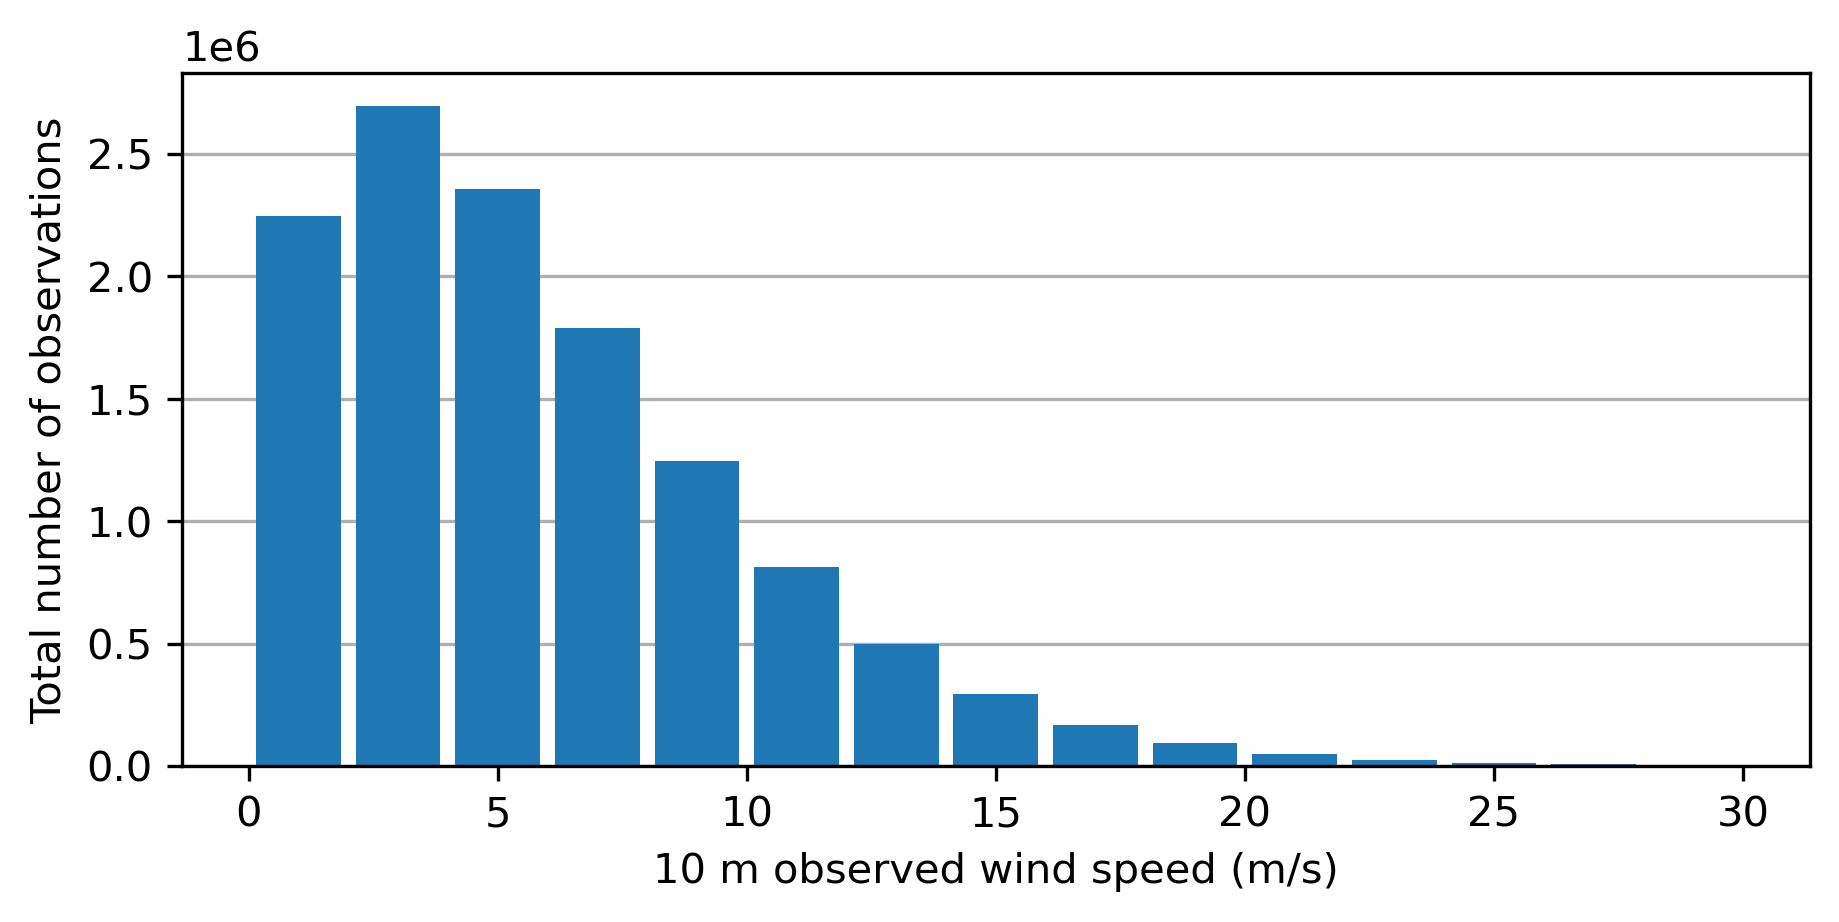
\includegraphics[width=\textwidth]{Figures/obs_wind_speeds.png}
        \label{fig:obs_wind_speeds}
    \end{subfigure}
    
    \vspace{0.5cm} % Space between the two images

    % Second subfigure (bottom)
    \begin{subfigure}[b]{0.8\textwidth}
        \centering
        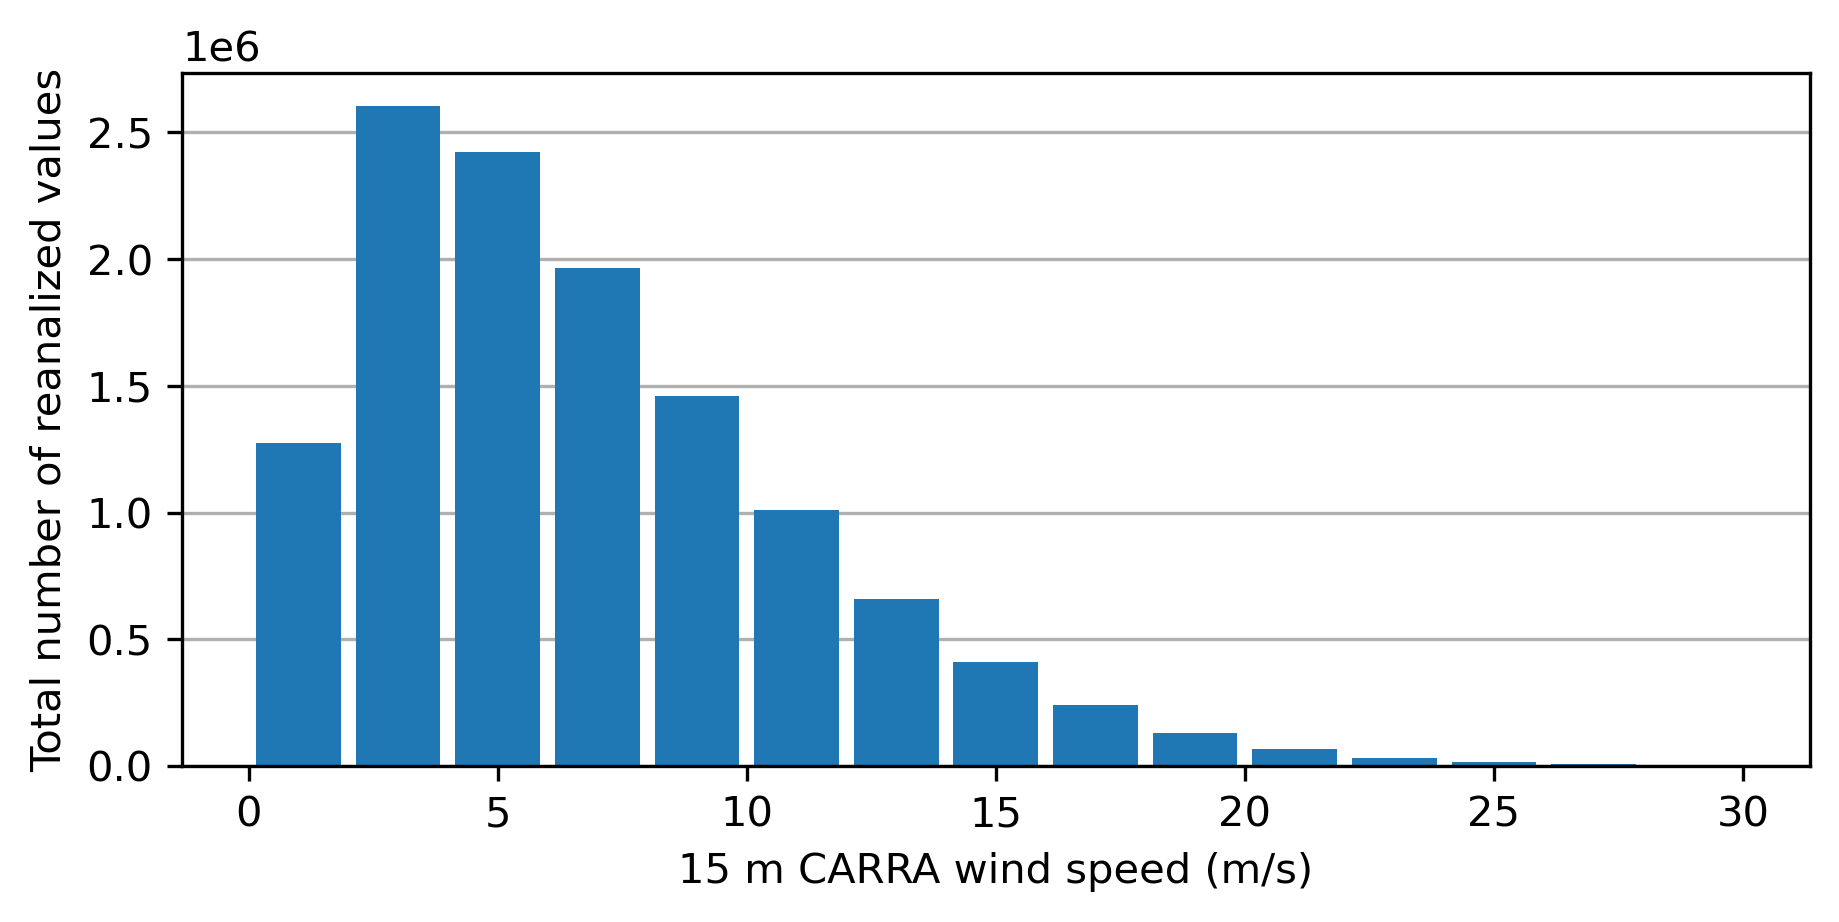
\includegraphics[width=\textwidth]{Figures/carra_wind_speeds.png}
        \label{fig:carra_wind_speeds}
    \end{subfigure}

    \caption[Distribution of CARRA and observed wind speeds]{Upper figure shows a histogram of observed wind speeds provided by IMO and IRCA for all used weather stations. Lower figure shows the interpolated CARRA reanalysis values at weather stations. The reanalysis data is only available at 3 hour intervals and 2.5km grid. As such the observed values are only chosen at these specific times (00, 03, 06, ..., 21). Spatial interpolation is needed and is linearly weighted based on distance of CARRA grid points from stations.}
    \label{fig:obs_carra_wind_speeds}
\end{figure}

\begin{figure}[ht]
    \centering
    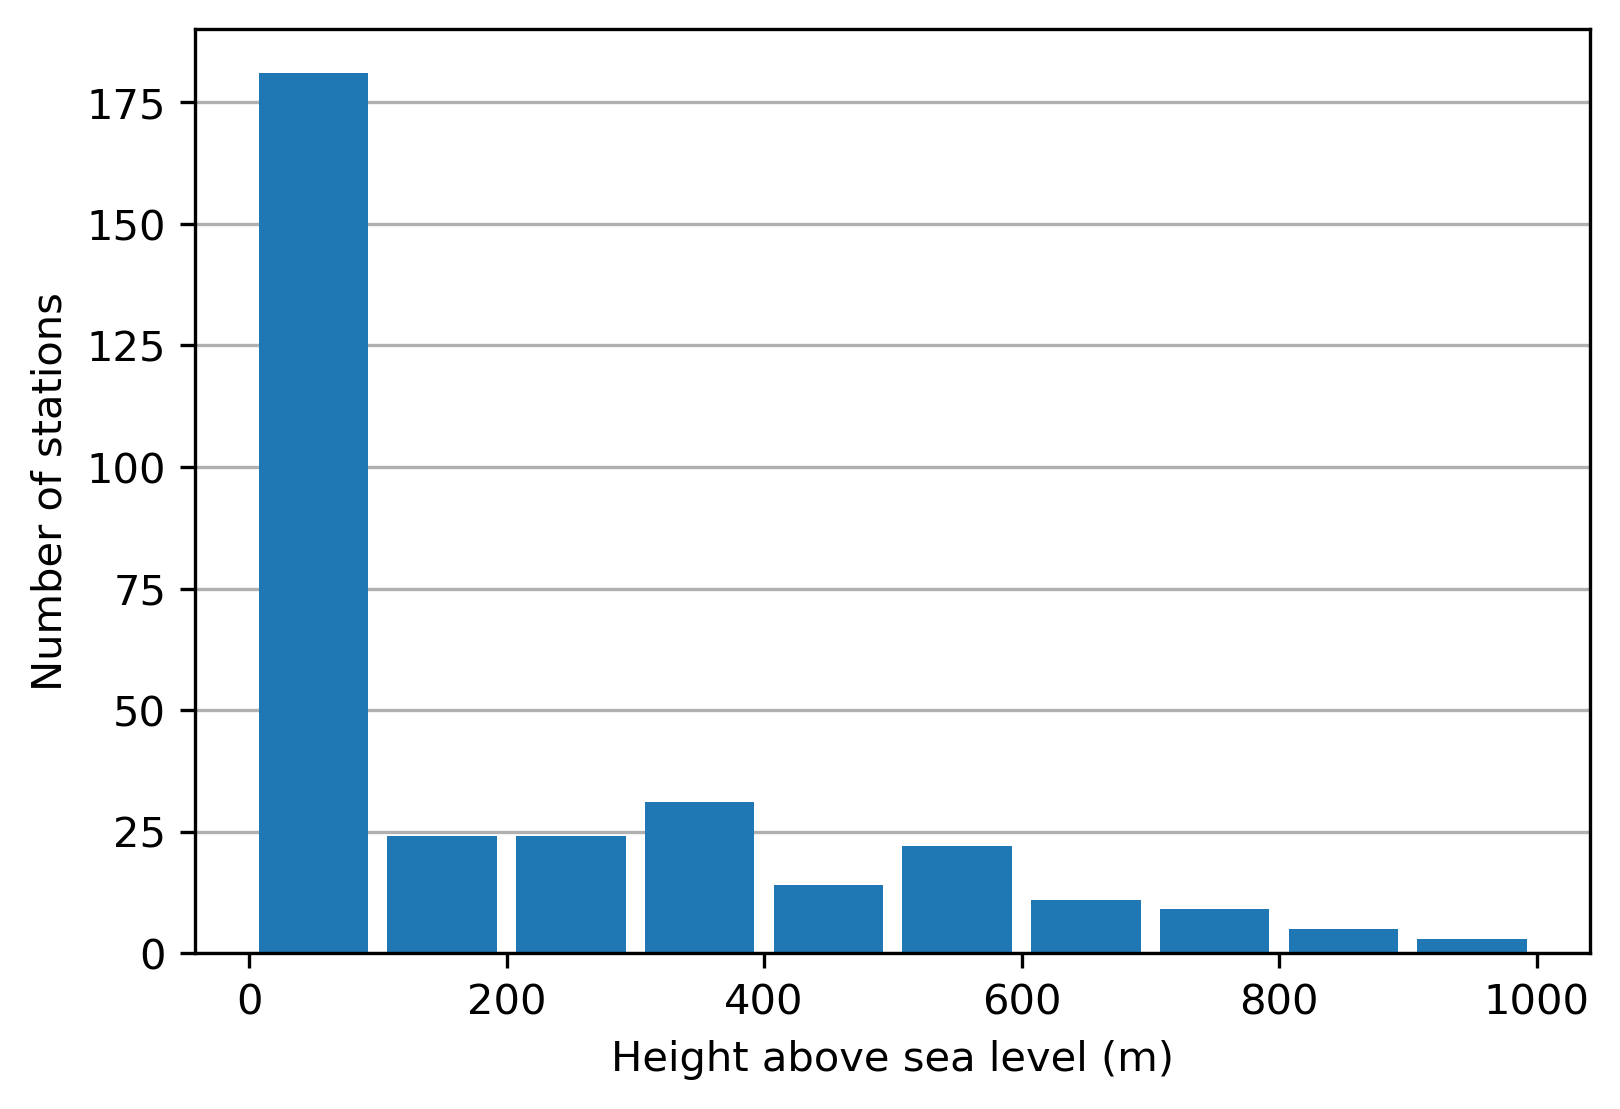
\includegraphics[width=0.8\textwidth]{Figures/station_heights.png}
    \caption[Distribution of weather station heights above sea level]{Distribution of heights of weather stations above sea level. One station has been excluded as an outlier of well above 1000 meters, having few and inconsistent datapoints.}
    \label{fig:station_heights}
\end{figure}

\begin{figure}[ht]
    \centering
    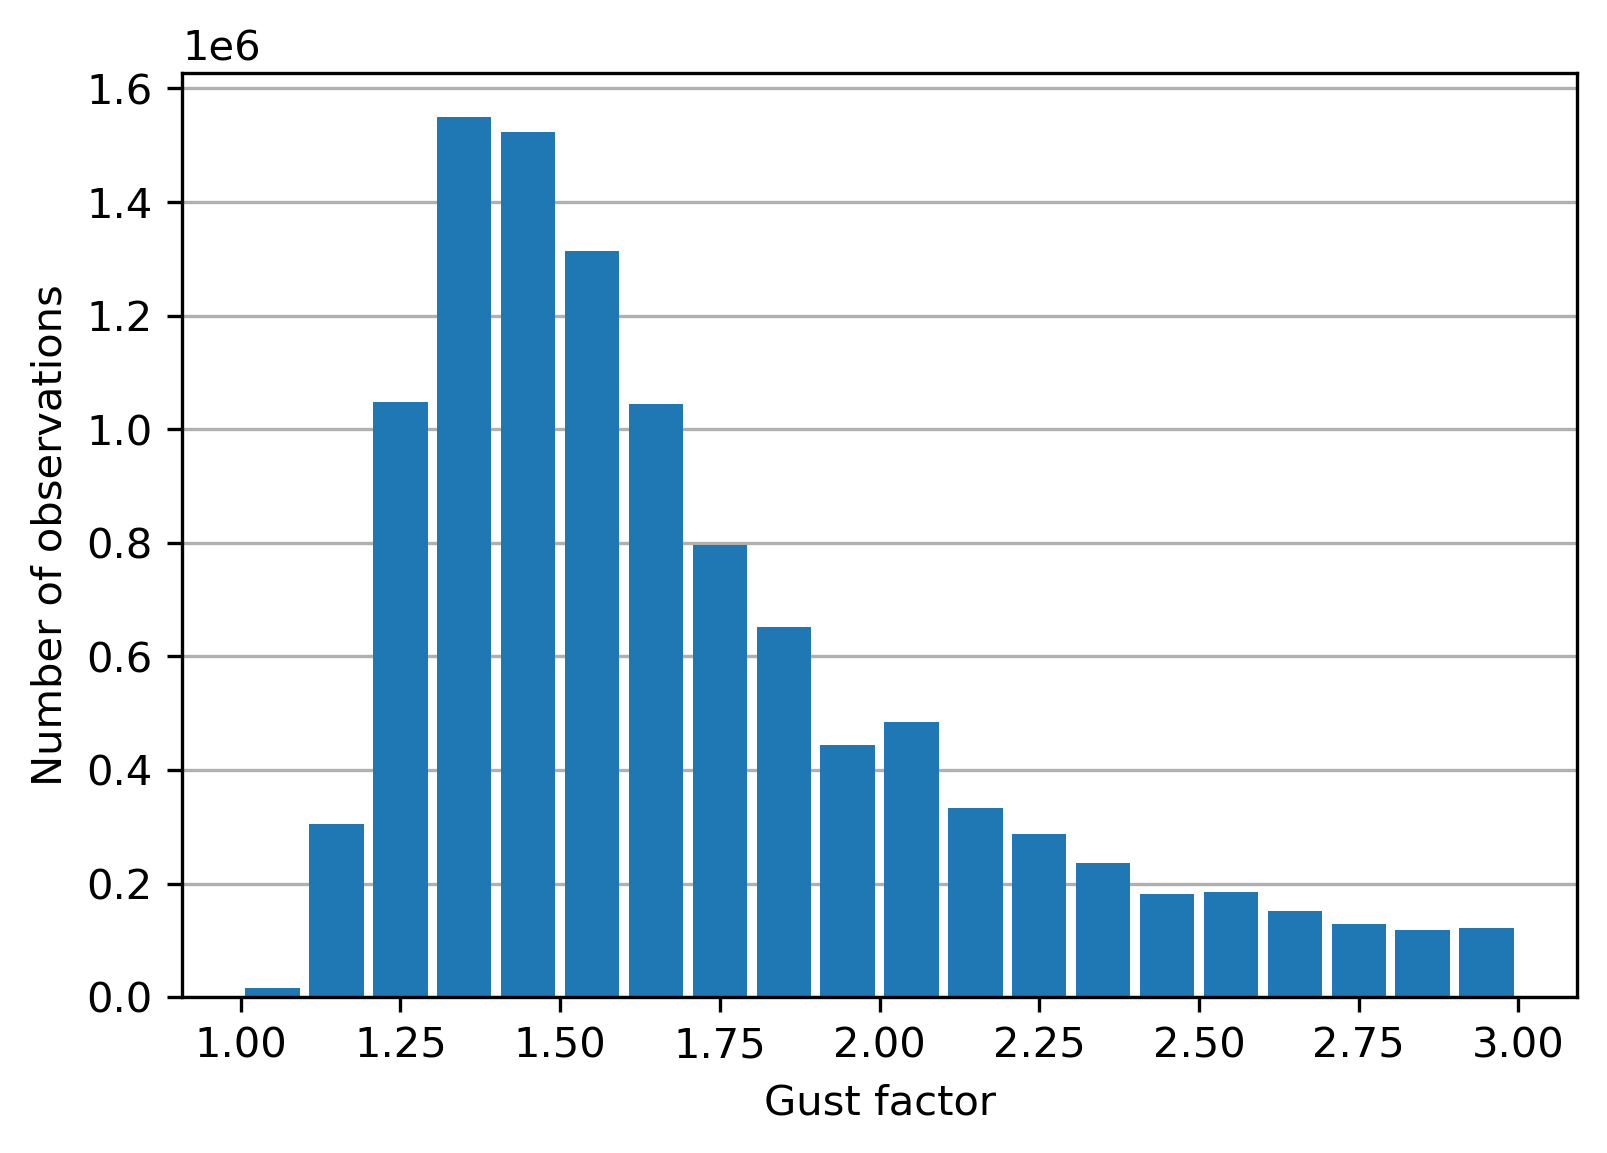
\includegraphics[width=0.8\textwidth]{Figures/gust_factor_2025.png}
    \caption[Distribution of gust factors]{Histogram of gust factors. By definition the lower bound of gust factor is 1. The majority of observed gust factors fall in the range 1.2 to 2. Gust factor decreases with increasing wind speed.}
    \label{fig:gust_factors}
\end{figure}

